\pdfobjcompresslevel=0
\documentclass[10pt,a4paper]{article}
\usepackage[utf8]{inputenc}
\usepackage[T1]{fontenc}
\usepackage{lmodern}
\usepackage{amsmath}
\usepackage[margin=1.2cm,top=1.0cm,bottom=1.0cm]{geometry}
\usepackage{booktabs}
\usepackage{fancyvrb}
\usepackage{graphicx}

\providecommand{\rocomma}[1]{{\ooalign{\null#1\crcr\hidewidth\raise-.31ex\hbox{\scriptsize,}\hidewidth}}}
\DeclareUnicodeCharacter{0218}{\rocomma{S}}
\DeclareUnicodeCharacter{0219}{\rocomma{s}}
\DeclareUnicodeCharacter{021A}{\rocomma{T}}
\DeclareUnicodeCharacter{021B}{\rocomma{t}}
\DeclareUnicodeCharacter{2013}{--}
\DeclareUnicodeCharacter{2014}{---}

\pagestyle{empty}
\setlength{\parindent}{0pt}
\setlength{\parskip}{2pt}
\setlength{\tabcolsep}{2.2pt}

\newcommand{\taskheading}[1]{\vspace{3pt}{\normalsize\bfseries #1}\par\vspace{1pt}}

\begin{document}
\small

{\large\bfseries Lab 04 — Filogenetică (\texttt{TP53}, secvența codificatoare) \hfill Paul Hondola}\par\vspace{2pt}
{\footnotesize\textbf{Dataset propriu} (\texttt{data/tp53\_cds.fasta}, NCBI RefSeq, doar CDS — UTR-urile au lungimi foarte diferite și ar domina distanțele):
Hsa \emph{Homo sapiens} NM\_000546.6 (1182 nt), Ptr \emph{Pan troglodytes} XM\_001172077.6 (1182), Mml \emph{Macaca mulatta} NM\_001047151.2 (1182),
Mmu \emph{Mus musculus} NM\_011640.3 (1173), Rno \emph{Rattus norvegicus} NM\_030989.4 (1176), Cfa \emph{Canis lupus familiaris} NM\_001389218.1 (1146),
Bta \emph{Bos taurus} NM\_174201.2 (1161), Ssc \emph{Sus scrofa} NM\_213824.3 (1161), Gga \emph{Gallus gallus} NM\_205264.1 (1104),
Xtr \emph{Xenopus tropicalis} NM\_001001903.1 (1089), Dre \emph{Danio rerio} NM\_131327.2 (1122), Ola \emph{Oryzias latipes} NM\_001104742.1 (1059).}\par
\vspace{2pt}\hrule\vspace{2pt}

\taskheading{Task 1 — Matrice de distanțe (3p)}
\begin{minipage}[t]{0.54\textwidth}\vspace{0pt}
\scriptsize
\begin{tabular}{l*{11}{c}}
\toprule
 & \textbf{Hsa} & \textbf{Ptr} & \textbf{Mml} & \textbf{Mmu} & \textbf{Rno} & \textbf{Cfa} & \textbf{Bta} & \textbf{Ssc} & \textbf{Gga} & \textbf{Xtr} & \textbf{Dre} \\ \midrule
\textbf{Ptr} & .003 &  &  &  &  &  &  &  &  &  &  \\
\textbf{Mml} & .036 & .037 &  &  &  &  &  &  &  &  &  \\
\textbf{Mmu} & .194 & .192 & .200 &  &  &  &  &  &  &  &  \\
\textbf{Rno} & .193 & .190 & .200 & .095 &  &  &  &  &  &  &  \\
\textbf{Cfa} & .155 & .157 & .163 & .228 & .231 &  &  &  &  &  &  \\
\textbf{Bta} & .167 & .169 & .172 & .223 & .249 & .188 &  &  &  &  &  \\
\textbf{Ssc} & .146 & .146 & .150 & .190 & .212 & .167 & .138 &  &  &  &  \\
\textbf{Gga} & .401 & .403 & .414 & .443 & .459 & .403 & .403 & .399 &  &  &  \\
\textbf{Xtr} & .378 & .381 & .379 & .378 & .373 & .383 & .423 & .376 & .414 &  &  \\
\textbf{Dre} & .420 & .408 & .408 & .419 & .415 & .421 & .430 & .397 & .448 & .423 &  \\
\textbf{Ola} & .440 & .433 & .448 & .437 & .453 & .486 & .454 & .450 & .537 & .441 & .362 \\
\bottomrule
\end{tabular}
\end{minipage}\hfill
\begin{minipage}[t]{0.44\textwidth}\vspace{0pt}\raggedright
Cele 66 de perechi au fost aliniate global cu \texttt{PairwiseAligner} ($+1/{-1}/{-2}$, ca în Lab 02); \emph{p}-distance pe coloanele fără gap și fără baze ambigue, apoi corecția \textbf{Jukes–Cantor} $d=-\tfrac34\ln(1-\tfrac43p)$: la $p\approx0.38$ (pește–pasăre) diferențele brute subestimează substituțiile multiple.
Tabelele complete: \texttt{results/distance\_matrix\_paulhondola.csv} și \texttt{pairwise\_paulhondola.csv}.
Cea mai apropiată pereche: \textbf{Hsa–Ptr}, $d=0.0025$ (3/1182 diferențe); cea mai îndepărtată: \textbf{Gga–Ola}, $d=0.5367$.
\end{minipage}

\taskheading{Task 2 — Arbore Neighbor-Joining (4p) și Bonus — vizualizare (+1p)}
\begin{minipage}[t]{0.52\textwidth}\vspace{0pt}
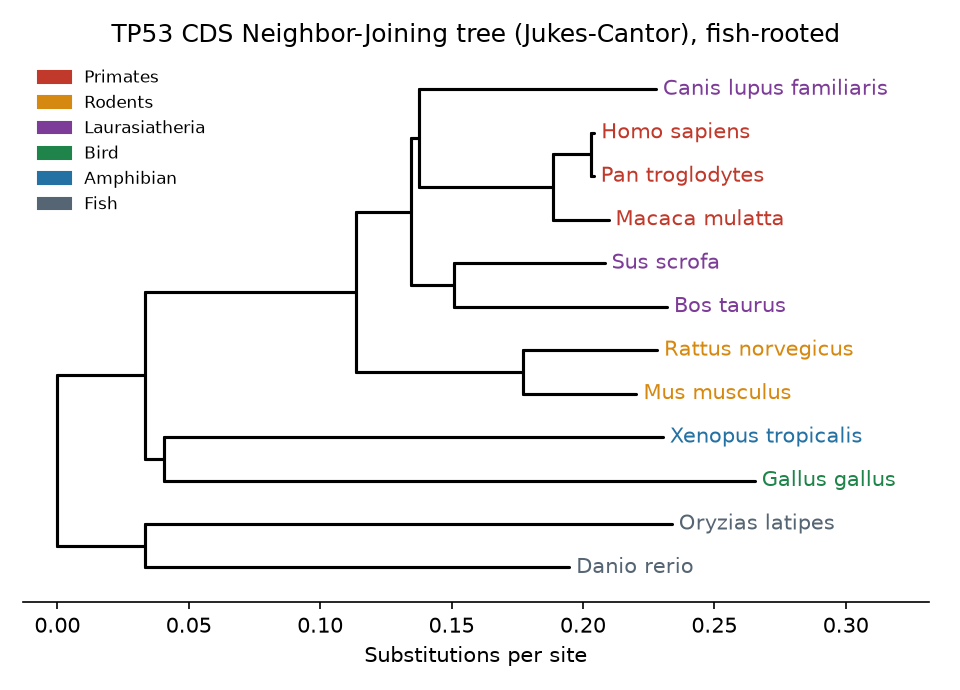
\includegraphics[width=\linewidth]{../../results/tree_paulhondola.png}
\end{minipage}\hfill
\begin{minipage}[t]{0.46\textwidth}\vspace{0pt}\raggedright
\texttt{DistanceTreeConstructor().nj()} pe matricea JC; NJ dă un arbore neînrădăcinat, înrădăcinat pe peștii Dre+Ola (care formează un clade), salvat în \texttt{results/tree\_paulhondola.nwk}; figura: \texttt{matplotlib} (\texttt{Bio.Phylo.draw}).
\textbf{Clustere:} (1) \emph{primate} (Hsa–Ptr aproape identice, Mml alături); (2) \emph{rozătoare} (Mmu–Rno, ramuri lungi: evoluție accelerată la rozătoare); (3) \emph{Cetartiodactyla} (Bta+Ssc); (4) \emph{mamifere} și \emph{tetrapode} monofiletice; (5) peștii ca outgroup.
\textbf{Abateri de la arborele speciilor:} câinele (Laurasiatheria) se grupează cu primatele pe o ramură internă foarte scurtă (0.003) — semnal slab într-o singură genă, nu o relație reală; găina se grupează cu broasca, deși păsările sunt sora mamiferelor (amniote): ambele au ramuri lungi și distanțe saturate ($d\approx0.4$), iar NJ le „atrage” împreună (\emph{long-branch attraction}). Arborele unei gene nu este arborele speciilor.
\end{minipage}

\taskheading{Task 3 — Comparație cu Clustal Omega (EBI) și regiuni conservate (3p)}
MSA online (\texttt{data/clustalo\_msa.aln}) și arborele lui Clustal Omega (\texttt{data/clustalo\_phylotree.nwk}), construit din MSA, independent de aliniamentele noastre pe perechi.
\textbf{Robinson–Foulds} (bipartiții neînrădăcinate): $RF=2$, normalizat \textbf{0.11} — 8 din 9 bipartiții comune. Singura diferență este poziția broaștei: noi avem \{Gga, Xtr\}, Clustal are \{Dre, Ola, Xtr\}. Ambele metode recuperează primatele, rozătoarele, mamiferele și tetrapodele și ambele pun câinele lângă primate; baza tetrapodelor este partea instabilă a arborelui.
\textbf{Regiuni conservate:} 266/1236 coloane (21.5\%) sunt identice la toate 12 speciile, dar cel mai lung segment identic are doar 8 nt, deoarece a treia poziție a codonilor variază (mutații sinonime). Am marcat ferestrele de 30 de coloane cu $\geq60\%$ coloane identice (de $\sim$3 ori fondul) — 4 regiuni, toate în domeniul de legare la ADN (codoni $\sim$94–292, coordonate Hsa): \textbf{117–127} (bucla L1, K120), \textbf{169–179} (L2, R175), \textbf{235–258} (L3, M246/R248/R249), \textbf{270–281} (R273, R280) — exact reziduurile care ating ADN-ul și hotspot-urile de mutații din cancer. Sunt conservate prin selecție purificatoare: o substituție aici anulează legarea la ADN, deci funcția de supresor tumoral.

\begin{minipage}[t]{0.47\textwidth}\vspace{0pt}
\begin{Verbatim}[fontsize=\scriptsize]
Hsa  TTTGAGGTGCGTGTTTGTGCCTGTCCTGGGAGAGA
Mmu  TTTGAGGTTCGTGTTTGTGCCTGCCCTGGGAGAGA
Gga  TTCGAGGTGCGCGTGTGCGCATGTCCGGGGAGGGA
Xtr  TTTGAGGTTCGTGTGTGCGCCTGCCCCGGGAGGGA
Dre  TTTGAGGTGCGTGTGTGTGCATGTCCAGGCAGAGA
Ola  TTYGAGGTCAGAATCTGTGCTTGCCCGGGGCGGGA
(12) ** *****  *  * ** ** ** ** **  * **
\end{Verbatim}
\end{minipage}\hfill
\begin{minipage}[t]{0.51\textwidth}\vspace{0pt}\raggedright
\footnotesize Extras din regiunea 270–281 (6 din 12 rânduri; \texttt{*} = identic la toate 12). Tiparul \texttt{** **} arată că pozițiile 1–2 ale codonilor sunt păstrate, iar a treia variază: proteina e conservată mai mult decât ADN-ul (ex. R273 = \texttt{CGT} la mamifere, \texttt{AGA} la Ola — tot arginină).
MSA ajută față de perechi: plasează toate secvențele în aceleași coordonate, deci „conservat” înseamnă conservat la toate speciile simultan.
\end{minipage}

\end{document}
